\label{chapter:models}
Metamodels approximate the initial evaluation model by 
utilising a data-driven approach, which is based on 
statistical analysis of the observed data. Consequently, the 
selection of a suitable surrogate model is essential in the optimal 
utilization of MAEA-based optimization. In attempt to achieve 
homogeneity throughout this thesis, it is reminded that 
the observations' matrix formed of $n_{t}$ training 
patterns is denoted by $\mathbf{X} = [\vec{χ}_{1}, 
\vec{χ}_{2}, \hdots, \vec{χ}_{n_{t}}]^T$, where each 
component $\vec{χ}_{i} = [χ_{i,1}, χ_{i,2},\hdots, 
χ_{i,n_{β}}]$ represents an observation $\vec{χ} \in \mathbb{R}
^{n_{β}}$. Their corresponding objective function
values are included in matrix $\mathbf{F}(\vec{χ}) = 
[\vec{f}_{1}, \vec{f}_{2}, \hdots, \vec{f}_{n_{t}}]^{Τ}$, 
where each component $\vec{f}_{i} = [f_{i,1}, f_{i,2}, 
\hdots, f_{i,n}]$ represents a response $\vec{f} \in 
\mathbb{R}^{n_{β}}$. In order to simplify the mathematical 
equations describing the surrogate models, $\mathbf{F}
(\vec{χ})$ is reduced to an 1-dimensional matrix  by 
assuming, without loss in generality, that the optimization 
process has a single objective. From there, the 
respective equations describing a MOO can be easily formulated by 
combining the SOO equations iteratively for $n$ objectives. In 
SOO, therefore, $\mathbf{F}(\vec{χ}) \!= \!\mathbf{F} \!= [f_{1}, 
f_{2}, \hdots, f_{n_{t}} ]^{T} \!\in \!\mathbb{R}^{n_{t}}$. 
Surrogate models are used to predict the objective function value 
$f(\vec{β})$ at any untried location of the design space, i.e. at 
each candidate solution $\vec{β} \in \mathbb{R}^{n_{β}}$. 
The theoretical background of every metamodel utilized via SMT in 
this thesis is subsequently presented. 


\vfill
\section{Kriging}
Kriging\cite{Kriging} is a surrogate model used for 
predicting the objective function value at any candidate
solution $\vec{β} \in \mathbb{R}^{n_{β}}$ in the design space. 
In order to make the prediction Kriging uses an interpolation 
method that combines a deterministic term with the realization of 
stochastic process. The former is replaced by a regression model 
and the latter is the realization of the stationary process 
Gaussian $z(\vec{β}) \!\backsim \!N(0,C)$ with a zero mean 
and a covariance kernel $C(\vec{β})$ of the observations:
\begin{equation}
C(\vec{χ}_{i}, \vec{χ}_{j}) = σ^{2} R(\vec{χ}_{i}, \vec{χ_{j}})
\end{equation} 
\\[-0.5cm]
where $σ^2$ the variance of the process and $R( \vec{χ_{i}}, 
\vec{χ_{j}})$ the correlation between any two observations
$\vec{χ_{i}}, \vec{χ_{j}} \!\in \!\mathbb{R}^{n_{β}}, \forall i,j 
\in [1,n_{t}]$. In order to improve the fitting of the Kriging 
model the distribution of training patterns in each problem 
dimension is normalized:
\begin{equation}
\vec{χ}_{norm} = \dfrac{\vec{χ} - μ_{\vec{χ}^{(j)}} }
{σ_{\vec{χ}^{(j)}}}
\end{equation} 

\newpage
%------------------------------------------------------------

\vspace{1mm} 
where $\vec{χ}^{(j)} \!= \! [χ_{1,j}, χ_{2,j}, 
\hdots, χ_{n_{t},j} ]^{T} \! \in \! \mathbb{R}^{n_{t}}$ is the 
column vector of the $n_{t} \times n_{β}$ matrix $\mathbf{X}$ 
and $μ_{\vec{χ}^{(j)}}$, ${σ_{\vec{χ}^{(j)}}}$ the mean 
value and the standard deviation of the $j_{th}$ observation, 
respectively. The correlation between any normalized 
training point $\vec{{χ}}_{norm} \!\in \!S \!\subset \!\mathbb{R}
^{n_{β}}$, where $S$ is the design set, can be computed using one 
of the following correlation kernels \footnote{In all Kriging 
models from this point on, the notation of normalization will not 
be used for sampled points but will be implied for simplicity, so 
$\vec{χ} \equiv \vec{{χ}}_{norm}$ and $\vec{χ} \equiv \vec{{χ}}
_{norm}$} \cite{preprint_SMT,Matern}:

\begin{itemize}
\item Exponential Ornstein-Uhlenbeck process
\begin{equation}\label{Oberstein correlation}
R \left( \vec{χ_{i}}, \vec{χ_{j}} \right) = 
\prod_{l=1}^{n_{β}}exp \left( -\theta_{l} 
\left| χ_{i,l} - χ_{j,l} \right| \right)
\end{equation}
              
\item Gaussian
\begin{equation}\label{Gaussian correlation}
R \left( \vec{χ_{i}}, \vec{χ_{j}} \right)  = 
\prod_{l=1}^{n_{β}}exp \left(-\theta_{l} 
\left( χ_{i,l} - χ_{j,l} \right)^2  \right)
\end{equation}  

\item Mat\'ern 5/2
\begin{equation}
R \left( \vec{χ_{i}}, \vec{χ_{j}} \right)  = 
\prod_{l=1}^{n_{β}} \left(\! 1 + \sqrt{5}\left|χ_{i,l} -
χ_{j,l} \right| + \dfrac{5}{3} θ_{l}^2\left( χ_{i,l} -
χ_{j,l} \right)^2 \right)\! exp\! \left(\!-\sqrt{5}θ_{l} 
\left| χ_{i,l} - χ_{j,l} \right|\right)
\end{equation}

\item Mat\'ern 3/2
\begin{equation}
R \left( \vec{χ_{i}}, \vec{χ_{j}} \right)  = 
\prod_{l=1}^{n_{β}} \left(\! 1 + \sqrt{3} θ_{l}
\left|χ_{i,l} - χ_{j,l} \right| \right) 
exp\! \left(\!-\sqrt{3}θ_{l} \left| χ_{i,l} - χ_{j,l} 
\right|\right)
\end{equation}
\end{itemize}
\vspace{1mm}
where $θ_{l}$ are parameters that denote the degree of 
correlation between training points w.r.t. each design 
dimension $l \in [1,n_{β}]$. Kriging assumes that the estimated 
value of each correlation parameter $θ$ is constant for each 
independent design variable and therefore for each design 
dimension, leading to the creation of an isotropic 
model\cite{Kriging1}. The correlation patterns of the observed 
data and their corresponding covariance can be stated in the form 
of an orthogonal matrix $\mathbf{R}$ and $\mathbf{C}$, 
respectively:
\begin{equation}
\textbf{R} = 
	\begin{bmatrix}
	R(\vec{χ}_{1}, \vec{χ}_{1}) & \hdots & 
	R(\vec{χ}_{1}, \vec{χ}_{n_{t}})
	\\
	\vdots & \ddots & \vdots
	\\
	R(\vec{χ}_{n_{t}}, \vec{χ}_{1}) & \hdots & 
	R(\vec{χ}_{n_{t}}, \vec{χ}_{n_{t}})
	\end{bmatrix} 
, \hspace{3mm} \mathbf{C} = 
\begin{bmatrix}
	C(\vec{χ}_{1}, \vec{χ}_{1}) & \hdots & 
	C(\vec{χ}_{1}, \vec{χ}_{n_{t}})
	\\
	\vdots & \ddots & \vdots
	\\
	C(\vec{χ}_{n_{t}}, \vec{χ}_{1}) & \hdots & 
	C(\vec{χ}_{n_{t}}, \vec{χ}_{n_{t}})
\end{bmatrix}
\end{equation} 

Under the assumption of a SOO problem, the Kriging model computes 
the objective function value at any normalized point $\vec{β} \in 
\mathbb{R}^{n_{β}}$ outside the sampled design as such:
\begin{equation}\label{Kriging_model_function}
f(\vec{β}) = μ_{Κ} + z(\vec{β})
\end{equation}
\\[-0.4cm]
where the deterministic term  $μ_{Κ}$ is expressed as a constant, 
linear or quadratic regression model:
\begin{equation}\label{deterministic_term}
μ_{Κ} = \sum_{j=1}^{k} \mathrm{w}_{j} p_{j}(\vec{β})
\end{equation}

\newpage
%--------------------------------------------------------


where $\mathrm{w} _{j}$ is the $j_{th}$ regression coefficient and 
$p_{j}: \mathbb{R}^{n_{β}} \mapsto \mathbb{R}$ are $k$ chosen 
functions. The parameter $k$ assumes various values to denote a 
constant, a linear or a quadratic regression model 
\cite{regression_model}. In a constant regression model, $k=1$ and 
$p_{1}(\vec{β}) \!= \!1$.  In a linear regression model, $k \!= \!
n_{β}+ 1$ and the corresponding functions assume the following 
values:

\begin{equation}
p_{1}(\vec{β}) = 1, \hspace{1mm} p_{2}(\vec{β}) = β_{1}, \hdots, 
\hspace{1mm} p_{k}(\vec{β}) = β_{n_{β}} 
\end{equation}
\\[-0.22cm]
In a quadratic regression model, $k=\dfrac{1}{2}(n_{β}+1)
(n_{β}+2)$ and the functions $p_{j}$ assume the following values:
\begin{equation}
\begin{split}
& p_{1}(\vec{β}) = 1, \hspace{2mm} 
p_{2}(\vec{β}) = β_{1}, \hdots,
\\ &
p_{n_{β}+1}(\vec{β}) = β_{n_{β}}, \hspace{2mm}
p_{n_{β}+2}(\vec{β}) = β_{1}^{2}, \hdots,
\\ &
p_{2n_{β}+1}(\vec{β}) = β_{1} β_{n_{β}}, 
\hspace{2mm}
p_{2n_{β}+2}(\vec{β}) = β_{2}^{2}, \hdots,
\\ &
p_{3n_{β}}(\vec{β}) = β_{2} β_{n_{β}}, \hdots
\\&
p_{k}(\vec{β}) = β_{n_{β}}^2
\end{split}
\end{equation}
\\[-0.2cm]
where $β_{j}\! \in \!\mathbb{R}$ is the component of any untried
point $\vec{β} \hspace{1mm}$ w.r.t. the $j_{th}$ design dimension 
for $j\! \in\! [1,n_{β}]$. 

\vspace{0.6cm}

\begin{itemize}
\item \textbf{Prediction with noise-free observations}
\end{itemize}

Kriging, when provided with the observed data that are collected 
via the implementation of DoE, can predict the value of any 
individual at any untried location of the design space 
accompanied by the measure of confidence of the prediction at 
that location. Under the assumption of a SOO problem, consider 
the linear predictor $\hat{f}(\vec{β})$ of the objective function 
at any untried point $\vec{β}$, given the prior observations 
$\mathbf{F} = [\vec{f}_{1}, \vec{f}_{2}, \hdots, \vec{f}
_{n_{t}}]^{T}$:
\begin{equation}\label{initial_linear_predictor}
\hat{f}(\vec{β}) = \vec{c}^{\hspace{1mm} T}(β) \mathbf{F} 
\end{equation}
\\[-2mm]
where $\vec{c}(β) \in \mathbb{R}^{n_{t}}$ is the $n_{t} \times 1$ 
vector of coefficients. Then the deviation between the predictor 
and the true objective function value:
\begin{equation}\label{linear_predictor}
\begin{split}
\hat{f}(\vec{β}) - f(\vec{β})& =  
\vec{c}^{\hspace{1mm} T}(\vec{β}) \mathbf{F} - ( μ_{Κ} + 
z(\vec{β})) \xrightarrow[(\ref{deterministic_term})]
{(\ref{Kriging_model_function})}
\\ &
= \vec{c}^{\hspace{1mm} T}(\vec{β}) \left( \mathbf{P}
\vec{\mathrm{w}} + \mathbf{Z} \right) - 
( \vec{p}^{\hspace{1mm} T}(\vec{β}) \vec{\mathrm{w}} + z(\vec{β}) )
\\ &
= \vec{c}^{\hspace{1mm} T}(\vec{β}) \mathbf{Z} - z(\vec{β}) +
( \mathbf{P}^{T} \vec{c}(\vec{β}) - \vec{p}(\vec{β}) )^{T} 
\vec{\mathrm{w}} 
\end{split}
\end{equation}
\\[1mm]
where $\mathbf{Z} = [z_{1}, z_{2}, \hdots, z_{n_{t}}]^{T}$ is the 
$n_{t} \times 1$ vector of errors at the observed points, 
$z(\vec{β})$ is the error at the untried location,
$\vec{p}(\vec{β}) = [p_{1}(\vec{β}), p_{2}(\vec{β}), \hdots, 
p_{k}(\vec{β})]^{T}$ is the $k \times 1$ vector of the chosen 
functions at any untried input $\vec{β}$ and $\mathbf{P}$ the 
corresponding $n_{t} \times k$ matrix for the complete design of 
observed data, which for $i = 1,n_{t}$ training patterns $\vec{χ}
_{i} \! = \! [χ_{i,1}, χ_{i,2}, \hdots, χ_{i,n_{β}}] \! \in \! S 
\!\subset \!\mathbb{R}^{n_{β}}$ is expressed as:


\newpage
%------------------------------------------------------------


\begin{equation}\label{polynomial_matrix}
\mathbf{P} = 
\begin{bmatrix}
p_{1}(\vec{χ}_{1}) & p_{2}(\vec{χ}_{1}) & \ldots 
&  p_{k}(\vec{χ}_{1}) 
\\
p_{1}(\vec{χ}_{2}) & p_{2}(\vec{χ}_{2}) & \ldots 
&  p_{k}(\vec{χ}_{2}) 
\\
\vdots & \vdots & \ddots & \vdots 
\\
p_{1}(\vec{χ}_{n_{t}}) & p_{2}(\vec{χ}_{n_{t}}) & \ldots 
&  p_{k}(\vec{χ}_{n_{t}}) 
\end{bmatrix}
%=
%\begin{bmatrix}
%1 & χ_{1,1} & \ldots &  χ_{1,n_{β}} 
%\\
%1 & χ_{2,1} & \ldots &  χ_{2,n_{β}} 
%\\
%\vdots & \vdots & \ddots & \vdots 
%\\
%1 & χ_{n_{t},1} & \ldots &  χ_{n_{t},n_{β}} 
%\end{bmatrix}
\end{equation}
\\[-3mm]

The best linear unbiased predictor (BLUP) is obtained by 
selecting the vector $\vec{c}(\vec{β})$ that minimizes the mean 
squared error (MSE). In order to keep the predictor 
unbiased, we demand that the expected value of the predictor 
and objective function coincides at the design sites $\mathbf{X}$
\cite{BLUP}:
\begin{equation}\label{constraint_BLUP}
\begin{split}
& E[\hat{f}(\vec{β}) - f(\vec{β})] = 0 
\xrightarrow{(\ref{linear_predictor})}
E[\vec{c}^{\hspace{1mm} T}(\vec{β}) \mathbf{Z} - z(\vec{β}) +
( \mathbf{P}^{T} \vec{c}(\vec{β}) - \vec{p}(\vec{β}))^{T} 
\vec{\mathrm{w}} ] = 0 \rightarrow
\\ & 
\vec{c}^{\hspace{1mm} T}(\vec{β})E[\mathbf{Z}] - E[z(\vec{β})] +
E[( \mathbf{P}^{T} \vec{c}(\vec{β}) - \vec{p}(\vec{β}))^{T} 
\vec{\mathrm{w}} ] = 0 
\xrightarrow{E[z(\vec{β})] = μ_{z} = 0}
\\ &
E[( \mathbf{P}^{T} \vec{c}(\vec{β}) - \vec{p}(\vec{β}))^{T}] 
\vec{\mathrm{w}}  = 0 
\rightarrow
\mathbf{P}^{T} \vec{c}(\vec{β}) - \vec{p}(\vec{β}) = 0
\end{split}
\end{equation}
\\
Consequently, the MSE of the predictor is calculated as such:
\begin{equation}\label{BLUP_predictor}
\begin{split}
E[\hat{f}(\vec{β})] & = E[\hat{f}(\vec{β}) - f(\vec{β})]^2 =
E[( \vec{c}^{\hspace{1mm} T}(\vec{β}) \mathbf{Z} - z(\vec{β}) )^2]
\\ & =
E[\vec{c}^{\hspace{1mm} T}(\vec{β}) \mathbf{Z}\mathbf{Z}^{T} 
\vec{c}(\vec{β})]- 2\vec{c}^{\hspace{1mm} T}(\vec{β})\mathbf{Z}
z(\vec{β}) + z^2(\vec{β}) ]
\\ & =
σ^{2}\left( \vec{c}^{\hspace{1mm} T}(\vec{β}) \mathbf{R}\vec{c}
(\vec{β}) - 2\vec{c}^{\hspace{1mm} T}(\vec{β})\vec{r}_{Xβ} + 1 
\right)
\end{split}
\end{equation}
\\
where $\vec{r}_{Xβ} = [R(\vec{χ}_{1}, \vec{β}), R(\vec{χ}
_{2}, \vec{β}), \hdots, R(\vec{χ}_{n_{t}}, \vec{β})]^{Τ}$ 
is the $n_{t} \times 1$ matrix denoting the correlation 
between the $n_{t}$ observations and any untried candidate solution 
$\vec{β} \! \in \!\mathbb{R}^{n_{β}}$.  $E[\hat{f}(\vec{β})]$ 
is minimized w.r.t. $c(\vec{β})$ and subject to the equality 
constraint $\mathbf{P}^{T} \vec{c}(\vec{β}) - \vec{p}(\vec{β})=0$ 
stated in eq. \ref{constraint_BLUP}, when the Kriging BLUP at some 
untried point $\vec{β} \in \mathbb{R}^{n_{β}}$ is given by equation 
\ref{Kriging_BLUP}: 

\begin{equation}\label{Kriging_BLUP}
\mathrm{\hat{f}}(\vec{β}) = 
\vec{p}^{\hspace{1mm} Τ}(\vec{β}) 
\hat{\vec{\mathrm{w}}} + \vec{r}_{Xβ}\mathbf{R}^{-1} 
\left(\mathbf{F} - \mathbf{P}\hat{\vec{\mathrm{w}}} 
\right)
\end{equation}
\\[-1mm]
The regression coefficients of the BLUP are estimated at the 
observed design sites using generalised least-squares method. The
$k \times 1$ vector $\hat{\vec{\mathrm{w}}} = [\mathrm{w}_{1},
\mathrm{w}_{2}, \hdots, \mathrm{w}_{k}]^{T}$ of the estimates of
$\vec{\mathrm{w}}$ are given by:
\begin{equation}\label{w_predictor}
\hat{\vec{\mathrm{w}}} = \left(\mathbf{P}^{T} 
\mathbf{R}^{-1}\mathbf{P}\right)^{-1} 
\mathbf{P}^{T} \mathbf{R}^{-1}\mathbf{F}
\end{equation}
\\[-4mm]
The MSE of the Kriging predictor can be computed using equation 
\ref{final_MSE_predictor}:
\begin{equation}\label{final_MSE_predictor}
MSE(\vec{β}) = \hat{σ}^{2}(1 -  \vec{r}_{Xβ}^{\hspace{1mm} Τ} 
\mathbf{R}^{-1}\vec{r}_{Xβ})
\end{equation} 
\\[-2mm]
which can be solved by adopting generalised least-squares estimates 
for the variance:

\begin{equation}\label{σ^2_predictor}
\widehat{σ}^{2} = \dfrac{1}{n_{t}} ( \mathbf{F} -
\mathbf{P}\hat{\vec{\mathrm{w}}} )^{T} 
\mathbf{R}^{-1} ( \mathbf{F} - \mathbf{P}
\hat{\vec{\mathrm{w}}} )
\end{equation}
\newpage
%----------------------------------------------------------------


The computation of the Kriging predictor requires the inversion
of the symmetric matrix of correlations $\mathbf{R}$, so the 
computational cost depends on the size of the training sample 
$n_{t}$. The calculation of $\mathbf{R} \!= \!\mathbf{R}(\vec{θ})$ 
requires the computation of $n_{β}$ correlation parameters $θ$, 
assuming an isotropic design, which are estimated using either 
maximum likelihood or cross validation method. The former method 
is more commonly used and dictates the selection of those 
parameters $θ$ that maximize the likelihood function $l_{F}(\vec{θ} 
| \mathbf{F})$ given the responses $\mathbf{F}$, which is a 
function of $\vec{θ} = [θ_{1}, θ_{2}, \hdots, θ_{n_{β}}]$ 
mathematically expressed as \cite{max_likelihood}:

\begin{equation}
l_{F}(\vec{θ} | \mathbf{F}) = 
\dfrac{1}{(2π)^{n_{t}/2} (σ^2)^{n_{t}/2} det\mathbf{R}^{1/2} }
exp \left[ \dfrac{-( \mathbf{F} - \mathbf{P}\hat{\vec{\mathrm{w}}} 
)^{T} 
\mathbf{R}^{-1} ( \mathbf{F} - \mathbf{P}
\hat{\vec{\mathrm{w}}} )}{σ^2} \right]
\end{equation}
\\
Intuitively, this process tries to infer the design space 
population that is most likely to have generated the responses 
$\mathbf{F}$. The complexity of the previous equation decreases by 
computing $ln(l_{F}(\vec{θ} | \mathbf{F}))$, since $ln(\cdot)$ is 
monotonous: 

\begin{equation}\label{likelihood_fun}
\begin{split}
ln(l_{F}(\vec{θ} | \mathbf{F})) = & - \dfrac{n_{t}}{2}ln(2π) 
- \dfrac{n_{t}}{2}ln(σ^2) - \dfrac{1}{2}ln(det\mathbf{R}) 
\\ &
- \dfrac{ ( \mathbf{F} -\mathbf{P}\hat{\vec{\mathrm{w}}} )^{T} 
\mathbf{R}^{-1} ( \mathbf{F} - \mathbf{P}
\hat{\vec{\mathrm{w}}} ) }{σ^2}
\end{split}
\end{equation}
\\
After inserting equations \ref{w_predictor} and 
\ref{σ^2_predictor} in eq. \ref{likelihood_fun}, the latter 
can be written in the concentrated ln-likelihood form where any 
constant terms are ignored:
\begin{equation}\label{max_likelihood_fun}
\begin{split}
ln(l_{F}(\vec{θ} | \mathbf{F})) = & 
-\dfrac{n_{t}}{2} ln \left[
\dfrac{1}{n_{t}} \left( \mathbf{F} - \mathbf{P} (\mathbf{P}^{T} 
\mathbf{R}^{-1}\mathbf{P})^{-1} 
\mathbf{P}^{T}\mathbf{R}^{-1}\mathbf{F} \right)^{T}
\right.
\\ & \times \left.  
\mathbf{R}^{-1} \left( \mathbf{F} - \mathbf{P} 
\left(\mathbf{P}^{T} \mathbf{R}^{-1}\mathbf{P}
\right)^{-1} \mathbf{P}^{T}\mathbf{R}^{-1}\mathbf{F}
\right) \right] + ln(det\mathbf{R} )
\end{split}	
\end{equation}
\\
Due to the dependency on the correlation $\mathbf{R}(\vec{θ})$ on 
the number of training patterns $n_{t}$, the cost of maximizing
$ln(l_{F}(\vec{θ} | \mathbf{F}))$, and therefore $l_{F}(\vec{θ} |
\mathbf{F})$, increases as the number of observations $n_{t}$ 
increases. In order to reduce the cost of solving this 
computationally expensive equation, a variety of algorithms are 
utilized, the most common of which is COBYLA algorithm (Constrained 
Optimization By Linear Approximation) \cite{COBYLA}, which uses 
linear approximations for the objective and constraint functions.



\newpage
%--------------------------------------------------------------

\begin{itemize}
\item \textbf{Prediction with noisy observations}
\end{itemize}

In the case of noisy predictions, the correlation matrix 
$\mathbf{R} \!\in \!\mathbb{R}^{n_{t} \times n_{t}}$ is no longer 
orthogonal, since the values in the leading diagonal of the matrix 
are not equal to 1 due to the introduced errors. In such a case, 
the least squares estimate given by equations \ref{w_predictor} and 
\ref{σ^2_predictor} will produce values that do not correspond to 
the physical model. In order to filter the noise, a parameter 
$λ_{R}$, referred to as nugget, is added to the leading diagonal of 
the matrix \cite{noisy data}. The nugget can be a vector $\vec{λ}
_{R} = [λ_{R_{1}}, λ_{R_{2}}, \hdots, λ_{R_{n_{t}}}]$ and vary for 
each observation or a scalar value $λ_{R}$ and be constant for all 
observations. Consequently, the correlation matrix $\mathbf{R}$ is
replaced by the term $\mathbf{R} + \vec{λ}_{R}I$ as such:

\begin{equation}
\begin{split}
& \mathrm{\hat{f}}(\vec{β}) =  
\vec{p}^{\hspace{1mm} Τ}(\vec{β}) 
\hat{\vec{\mathrm{w}}} + \vec{r}_{Xβ} 
(\mathbf{R} + \vec{λ}_{R}I)^{-1} 
\left(\mathbf{F} - \mathbf{P}\hat{\vec{\mathrm{w}}} 
\right)
\\ &
MSE(\vec{β}) = \hat{σ}^{2}(1 -  \vec{r}_{Xβ}^{\hspace{1mm} Τ} 
(\mathbf{R + \vec{λ}_{R}I})^{-1}\vec{r}_{Xβ})
\\ &
\hat{\vec{\mathrm{w}}} = \left(\mathbf{P}^{T} 
(\mathbf{R} + \vec{λ}_{R}I)^{-1}\mathbf{P}\right)^{-1} 
\mathbf{P}^{T} (\mathbf{R} + \vec{λ}_{R}I)^{-1} \mathbf{F}
\\ &
\widehat{σ}^{2} = \dfrac{1}{n_{t}} ( \mathbf{F} -
\mathbf{P}\hat{\vec{\mathrm{w}}} )^{T} 
(\mathbf{R} + \vec{λ}_{R}I)^{-1} ( \mathbf{F} - \mathbf{P}
\hat{\vec{\mathrm{w}}} )
\end{split}
\end{equation}
\\[-2mm]
where $I$ is the $n_{t} \times n_{t}$ identity matrix.

\newpage
%----------------------------------------------------------------

%we introduce the $k \times 1$ 
%vector of Lagrangian multipliers $\vec{κ}(\vec{β}) = [κ_{1}, 
%κ_{2}, \hdots, κ_{k}]^T$ and the corresponding Lagrangian 
%function: 

%\begin{equation}
%\begin{split}
%\mathfrak{L}\left( c(\vec{β}), \vec{κ}(\vec{β}) \right) & = 
%E[\hat{y}(\vec{β})] - \vec{κ}^{T}(\vec{β}) \left( \mathbf{P}^{T} 
%\vec{c}(\vec{β}) - \vec{p}(\vec{β}) \right)
%\\ & \overset{\ref{BLUP_predictor}}{=} 
%σ^{2}\left( \vec{c}^{\hspace{1mm} T}(β) \mathbf{R}\vec{c}(β) 
%- 2\vec{c}^{\hspace{1mm} T}(β)\vec{r}_{Xβ} + 1 \right)
%- \vec{κ}^{T}(\vec{β}) \left( \mathbf{P}^{T} \vec{c}(\vec{β}) - 
%\vec{p}(\vec{β}) \right)
%\end{split}
%\end{equation}
%\\[-3mm]
%The local minima of $E[\hat{y}(\vec{β})]$ that satisfy the 
%imposed constraint can be found by setting the partial derivative 
%of the Lagrangian function w.r.t. $c(\vec{β})$ equal to zero, 
%where the said partial derivative is:
%\begin{equation}\label{Lagrange_derivative}
%\dfrac{\partial \mathfrak{L}\left( c(\vec{β}), κ(\vec{β}) \right)}
%{\partial c(\vec{β})} = 2σ^{2} \left( \mathbf{R}
%c(\vec{β}) - \vec{r}_{Xβ}\right) - \mathbf{P}\vec{κ}(\vec{β}) = 0
%\end{equation}

%\newpage
%%----------------------------------------------------------------


%The Lagrangian multipliers and the coefficients of the BLUP must,
%therefore, satisfy equations \ref{constraint_BLUP} and 
%\ref{Lagrange_derivative}:

%\begin{equation}
%\begin{bmatrix}
%\mathbf{R} & \mathbf{P} \\
%\mathbf{P}^T & 0
%\end{bmatrix}
%	\begin{bmatrix}
%	\vec{c}(\vec{β}) \\ \vec{κ}^{\hspace{1mm} '}(\vec{β})
%	\end{bmatrix}
% =
%\begin{bmatrix}
%\vec{r}_{Xβ} \\ \vec{p}(\vec{β})
%\end{bmatrix}
%\end{equation}
%\\[-2mm]
%where $\vec{κ}^{\hspace{1mm} '}(\vec{β}) = $ \scalebox{0.9}{%$
%$- \dfrac{\vec{κ}(\vec{β})}{2σ^2}$} and the solution to the 
%previous equation is:
%\begin{equation}\label{Lagrange_solution}
%\begin{split}
%& \vec{κ}^{\hspace{1mm} '}(\vec{β}) = \left(\mathbf{P}^{T} 
%\mathbf{R}^{-1}\mathbf{P}\right)^{-1} 
%\left( \mathbf{P}^{T} \mathbf{R}^{-1}\vec{r}_{Xβ} - 
%\vec{p}(\vec{β}) \right)
%\\ &
%\vec{c}(\vec{β}) = \mathbf{R}^{-1} \left(\vec{r}_{Xβ} - 
%\mathbf{P} 
%\vec{κ}^{\hspace{1mm} '}(\vec{β}) \right)
%\end{split}
%\end{equation}
%\\[-1mm]
%Equation \ref{initial_linear_predictor} can then be restated as:
%\begin{equation}\label{predictor_mid}
%\begin{split}
%\hat{f}(\vec{β}) & =  \vec{c}^{\hspace{1mm} T}(β) \mathbf{F}
%\overset{\ref{Lagrange_solution}}{=} 
%\left(\vec{r}_{Xβ} - \mathbf{P} \vec{κ}^{\hspace{1mm} '}(\vec{β}) 
%\right)^{T} \mathbf{R}^{-1} \mathbf{F}
%\\ & =
%\vec{r}_{Xβ} \mathbf{R}^{-1} \mathbf{F} -
%\left( \mathbf{P}^{T} \mathbf{R}^{-1}\vec{r}_{Xβ} - 
%\vec{p}(\vec{β}) \right)^{T} 
%(\mathbf{P}^{T} \mathbf{R}^{-1}\mathbf{P})^{-1} 
%\mathbf{P}^{T} \mathbf{R}^{-1} \mathbf{F}
%\end{split}
%\end{equation}
%\\



\section{KPLS}  
In an attempt to decrease the construction time of Kriging
model in high-dimensional design spaces, the number of 
parameters $\vec{θ}$ is decreased via the use of Partial 
Least Squares (PLS) method\cite{PLS}. PLS is a 
statistical method used for observing the correlation 
between the design variables and the objective function 
by projecting the former in a design space of reduced 
dimensions $h$. This space is formed by $h$ parameters, 
which are called principal components or latent variables, 
and are linear combinations of the design variables. In KPLS 
\cite{KPLS}, the principal components $\mathbf{P_{c}} = 
[\vec{p_{c}}^{(1)}, \vec{p_{c}}^{(2)}, \hdots, \vec{p_{c}}^{(h)}]$ 
are retained via the implementation of the PLS method which seeks 
the best direction $\vec{D}^{(l)}$ that maximizes iteratively 
for $h$ reduced dimensions the covariance between 
$\vec{p}^{(l)}$ and $\mathbf{F}^{(l-1)}$, where $\mathbf{F}
^{(l-1)}$ are the responses at the observed design sites 
$\mathbf{X}^{(l-1)}$ for the $(l-1)_{th}$ principal component.

	\begin{equation}
	\vec{D}^{(l)} = 
	\underset{\vec{D}^{(l)}}{\mathrm{argmax}} 	
	\hspace{2mm}
	\vec{D}^{(l)^T} \mathbf{X}^{(l-1)^{T}} \mathbf{F}
	^{(l-1)} \mathbf{F}^{(l-1)^{T}} \mathbf{X}^{(l-1)} 
	\vec{D}^{(l)}  
	\hspace{2mm}, \text{for} \hspace{2mm} l=1,h
	\end{equation}
\\[-2mm]
which is maximized when $\vec{D}^{(l)^{T}} \vec{D}^{(l)} = 1$, i.e.
$\vec{D}^{(l)} = [D_{1}^{(l)}, D_{2}^{(l)}, \hdots, D_{n_{β}}
^{(l)}]^T$ is the $n_{β} \times 1$ eigenvector that corresponds 
to the scalar eigenvalue $λ_{eig} \in \mathbb{R}$ with the largest 
absolute value, which is estimated using the power iteration 
method proposed by Lanczos\cite{power_iter}. Let $\bm{Δ}^{(l-1)} 
\equiv \mathbf{X}^{(l-1)^{T}} \mathbf{F}^{(l-1)} \mathbf{F}
^{(l-1)^{T}} \mathbf{X}^{(l-1)}$, then each principal direction 
vector $\vec{D}^{(l)}$ maximizes the covariance of 
$\bm{Δ}^{(l-1)}$. For the first iteration of the algorithm, 
$\mathbf{X}^{(0)} \!\equiv \!\mathbf{X} \!\in \!\mathbb{R}^{n_{t} 
\times n_{β}}$ and $\mathbf{F}^{(0)} \!\equiv \!\mathbf{F} \!\in \!
\mathbb{R}^{n_{t}}$, assuming a SOO. With $D^{(l)}$ known, the 
principal component for the $l_{th}$ iteration can be calculated:

	\begin{equation}\label{direction_eq_h}
	\vec{p_{c}}^{(l)} = \mathbf{X}^{(l-1)} \vec{D}^{(l)}
	\end{equation}
\\[-3mm]
where $\vec{p_{c}}^{(l)} = [p_{c_{1}}^{(l)}, p_{c_{2}}^{(l)}, 
\hdots, p_{c_{n_{t}}}^{(l)}]^{T}$ is the $n_{t} \times 1$ principal 
component vector for the $l_{th}$ principal dimension.  
Subsequently, the matrices of the design space and its
response are calculated and will be used to compute the 
values in the next iteration. 
	\begin{equation}
	\begin{split}
	& \mathbf{X}^{(l)} = \mathbf{X}^{(l-1)} - 
	\vec{p_{c}}^{(l)} \vec{\mathrm{w}}_{x}^{(l)} \\
	& \mathbf{F}^{(l)} = \mathbf{F}^{(l-1)} - \mathrm{w}
	_{F}^{(l)} \vec{p_{c}}^{(l)} 
	\end{split}
	\end{equation}
\\[-2mm]
where $\vec{\mathrm{w}}_{x}^{(l)}$ and $\mathrm{w}_{F}^{(l)}$ are 
the regression coefficients of the $l_{th}$ principal component for 
the local regression of $\mathbf{X}$ and $\mathbf{F}$, 
respectively, with the former being a $1 \times n_{β}$  matrix and 
the latter a scalar.  Prior to the initialisation of the iterative 
process, matrices $\mathbf{X}, \mathbf{F}$ have been scaled 
and centered on the origin point of the initial coordinate 
system $O(0,0,\hdots,0)$; this has no impact on the correlation 
matrix $\mathbf{R}$. In addition, each resulting principal 
component is orthogonal to all the other principal components, 
since they compose the axes of the new coordinate system.

The completion of the iterative process results in the creation of 
a formatted design space of $h < n_{β}$ dimensions, which is 
defined by the coordinate system that the principal components form
and is created by rotation of the original design space.
This rotation can be quantified by the definition of a new
matrix\cite{rotation_matrix}:

\begin{equation}
\mathbf{D}_{*} = \mathbf{D} \left( \bm{W_{x}}^{Τ} 
\mathbf{D} \right)^{-1}
\end{equation}

\newpage
%--------------------------------------------------------------- 


In the previous equation, $\bm{W_{x}} = [\vec{\mathrm{w}_{x}}
^{(1)^{T}}, \vec{\mathrm{w}_{x}}^{(2)^{T}}, \hdots, \vec{\mathrm{w}
_{x}}^{(h)^{T}}]$ is the $n_{β} \times h$ matrix containing
the regression coefficients of $h$ principal components
for the local regression of $\mathbf{X}$ and $\mathbf{D} = [\vec{D}
^{(1)}, \vec{D}^{(2)}, \hdots, \vec{D}^{(h)}]$ is the $n_{β} 
\times h$ matrix of principal direction vectors. $\mathbf{D}_{*} 
\!= \![\vec{D}_{*}^{(1)}, \vec{D}_{*}^{(2)}, \hdots, \vec{D}_{*}
^{(h)}] \!\in \mathbb{R}^{n_{β} \times h}$ is obtained by restating 
eq. \ref{direction_eq_h} as such:

\begin{equation}
\vec{p_{c}}^{(l)} = \mathbf{X}^{(l-1)} \vec{D}^{(l)} = 
\mathbf{X}^{(0)} \mathbf{D}_{*}^{(l)}
\end{equation}
\\[-2mm]
where the scalar elements $D_{*1}^{(l)}, D_{*2}
^{(l)}, \hdots, D_{*n_{β}}^{(l)}$ in each vector $\vec{D}_{*}
^{(l)}$ measure the importance of each corresponding dimension 
in the construction of the $l_{th}$ principal component, where its
correlation with the response $\vec{f}$ is maximized. Respectively, 
the correlation parameters $\vec{θ} \! \in \!\mathbb{R}^{n_{β}}$ 
in Kriging quantify the importance of each dimension in the 
calculation of the respective response $\vec{f}$. The 
estimation of such parameters via maximization of the likelihood 
function in eq. \ref{max_likelihood_fun} is the most costly process 
of constructing the Kriging model. By assuming an isotropic and 
stationary process $R_{l}:S \times S \mapsto \mathbb{R}$, $\forall 
l \in [1,h]$, we can construct the KPLS kernel by using the 
scalar elements $D_{*1}^{(l)}, D_{*2}^{(l)}, \hdots, D_{*n_{β}}
^{(l)}$ to replace $\vec{θ}$ when measuring the importance of each 
one of the $n_{β}$ dimensions for the $l_{th}$ principal component. 
	\begin{equation}
	\begin{split}
	& R_{1:h} \left( \vec{χ_{i}}, \vec{χ_{j}} \right) = 
	\prod_{l=1}^{h} R_{l} \left(f_{c}^{(l)}(\vec{χ_{i}}), 
	f_{c}^{(l)}(\vec{χ_{j}}) \right), 
	\hspace{3mm}\text{with} \hspace{2mm} f_{c}^{(l)}: 
	S \mapsto S
	\\
	& \text{and} \hspace{2mm} 
	\begin{split}
	& \vec{χ_{i}} \longmapsto \left[ D_{*1}^{(l)} 
	χ_{i,1}, D_{*2}^{(l)} χ_{i,2}, \hdots, D_{*n_{β}}
	^{(l)} χ_{i,n_{β}}\right]
	\\
	& \vec{χ_{j}} \longmapsto \left[ D_{*1}^{(l)} 
	χ_{j,1}, D_{*2}^{(l)} χ_{j,2}, \hdots, D_{*n_{β}}
	^{(l)} χ_{j,n_{β}}\right]
	\end{split} 
	\end{split}
	\end{equation}
\\[-1mm]	
where $f_{c}^{(l)}$ denotes some correlation function defined in 
the rotated $n_{β}$-dimensional design space of $h$ principal 
components. This approach can be used to reconstruct two 
correlation kernels in order to decrease the number of parameters 
$θ \in \mathbb{R}^{h}$:

\begin{itemize}
\item Exponential Ornstein-Uhlenbeck process
\begin{equation}
R \left( \vec{χ_{i}}, \vec{χ_{j}} \right) = 
\prod_{l=1}^{h} \prod_{k=1}^{n_{β}} exp \left( -\theta_{l} 
\left| D_{*k}^{(l)}χ_{i,k} - D_{*k}^{(l)} χ_{j,k} \right| 
\right)
\end{equation}              

\item Gaussian
\begin{equation}\label{KPLS_Gaussian}
R \left( \vec{χ_{i}}, \vec{χ_{j}} \right)  = 
\prod_{l=1}^{h} \prod_{k=1}^{n_{β}} exp \left(-\theta_{l} 
\left( D_{*k}^{(l)} χ_{i,k} - D_{*k}^{(l)} χ_{j,k} 
\right)^2  \right)
\end{equation} 
\end{itemize}

The maximum likelihood given by eq.\ref{max_likelihood_fun} is 
subsequently estimated w.r.t. $θ \!\in \!\mathbb{R}^{h}$, thus 
significantly decreasing the computational cost. With $θ \!\in 
\!\mathbb{R}^{h}$ known, the correlation matrix is calculated and 
inserted in equations \ref{Kriging_BLUP} and 
\ref{final_MSE_predictor} that provide the KPLS prediction and the 
corresponding MSE.
\newpage
%-------------------------------------------------------


\section{KPLSK}
The KPLSK model is used for improving the maximum 
likelihood function of Kriging described by equation 
\ref{max_likelihood_fun}. This improved maximum likelihood 
function is obtained by following the construction process of KPLS 
model with one variation. After the values of parameters $θ$ have 
been calculated in the $h$-dimensional space via the use of KPLS 
model, KPLSK performs a local optimization of the likelihood 
function of Kriging by making it equivalent to the KPLS one 
\cite{KPLSK}. The idea is to express the KPLS kernels, which are 
defined in a subset of the $n_{β}$-dimensional space, in the 
entirety of the $n_{β}$-dimensional space. In the subset $S \subset 
\mathbb{R}^{n_{β}}$, the equivalence of the KPLS and Kriging 
kernels eq. \ref{KPLS_Gaussian} can be proved for exponential 
kernels of order $q$. In this case, $q = 2$ to refer to the 
Gaussian correlation kernel: 
\begin{equation}
\begin{split}
R \left( \vec{χ_{i}},\vec{χ_{j}} \right) 
& = \prod_{l=1}^{h} \prod_{k=1}^{n_{β}} exp \left(-
\theta_{l} \left( D_{*k}^{(l)} χ_{i,k} - D_{*k}^{(l)} 
χ_{j,k} \right)^2  \right)
\\
& = \prod_{l=1}^{h} \prod_{k=1}^{n_{β}} exp
\left(-θ_{l} D_{*k}^{(l)^2} 
\left( χ_{i,k} - χ_{j,k} \right)^2  \right)
\\
& = exp \left( \sum_{k=1}^{n_{β}} \sum_{l=1}^{h} \left(
-θ_{l} D_{*k}^{(l)^2} 
\left( χ_{i,k} - χ_{j,k} \right)^2 \right) \right)
\\
& = exp\left( \sum_{k=1}^{n_{β}} \left( -  
\hspace{2mm} η_{k}  \left( χ_{i,l} - χ_{j,l} \right)^2  
\right) \right)
\\
& = \prod_{k=1}^{n_{β}}exp \left( 
- η_{k} \left( χ_{i,k} - χ_{j,k} \right)^2 \right)
\end{split}
\end{equation}
\\[2mm]
Consequently, $η_{k}=\sum_{l=1}^{h} θ_{l} D_{*k}^{(l)^2}$ 
for $k=1,2,\hdots,n_{β}$ aids in the transition to the 
$n_{β}$-dimensional space, where it serves as a starting point for 
the local optimization of the Kriging likelihood function based on 
the values of parameters $θ^{(l)}$ obtained via the use of the KPLS 
method for $l = 1,2 \hdots, h$. 

\newpage
%------------------------------------------------


\section{Radial Basis Function (RBF)}
The comprehension of α RBF interpolation model initially 
requires defining radial functions. A function
$φ: \mathbb{R}^{n_{β}} \rightarrow \mathbb{R}$ is called
a radial function when its value at any given point 
$\vec{β} \in \mathbb{R}^{n_{β}}$ depends on the distance 
$r$ between that point and some other fixed point, called 
the center of the RBF and denoted by $c_{e}$\cite{RBF}.

\begin{equation}
φ(\vec{β}) = g(\lVert \vec{β} - \vec{c}_{e}\rVert) = g(r) 
\end{equation}
\\[-0.2cm]
where $\lVert \cdot \rVert$ denotes the Euclidean norm 
$\lVert \cdot \rVert_{2}$ and $g:[0,\infty) \rightarrow 
\mathbb{R}$ is a univariate radial basis function that depends 
solely on the distance $r$. The approximating model uses the 
$n_{t}$ observed pairs $(\vec{χ}, f(\vec{χ}))$ to yield the 
interpolant $s(\vec{β})$ at an untried point $\vec{β} \in 
\mathbb{R}^{n_{β}}$, which is a linear combination of 
RBFs\cite{RBF1} $g(r_{j})$, $\forall j \in [1,n_{t}]$.
\begin{equation}\label{RBF_equation}
\begin{split}
& s(\vec{β}) =\sum_{j=1}^{n_{t}} 
\mathrm{w}_{t_{j}} g \left( \lVert \vec{β} - \vec{χ}_{j} 
\rVert \right) =
\sum_{j=1}^{n_{t}} \mathrm{w}_{t_{j}} g(r_{j})
\\ &
\text{such that} \hspace{3mm} s(\vec{χ}_{i}) 
= F(\vec{χ}_{i}) = F_{i}
\hspace{5mm} ,\text{for} \hspace{2mm} i =1,n_{t}
\end{split}
\end{equation} 
\\[0.1cm]
where each observation $\vec{χ}_{j}$ serves as a center point for
the RBF $g(r_{j})$, with the distance between the $j_{th}$ 
interpolation center and the $i_{th}$ observation being equal to 
$r_{j} = \sqrt{(β_{1} - χ_{j,1})^{2} + (β_{2} - χ_{j,2})^{2} + 
\hdots + (β_{n_{β}} - χ_{j,n_{β}})^{2} }$. Each RBF is additionally 
weighted by an interpolation coefficient $\mathrm{w}_{t_{i}}$. The 
system described by eq. \ref{RBF_equation} is linear and solvable 
$\forall i,j \in [1,n_{t}]$:
\begin{equation}\label{RBF_no_poly}
\sum_{j=1}^{n_{t}} \mathrm{w}_{t_{j}} g
\left( \lVert \vec{χ}_{i} - \vec{χ}_{j} \rVert \right)  = 
F_{i} \hspace{5mm},\text{for} \hspace{2mm} i=1,n_{t}
\end{equation} 
\\[-0.2cm]
which in matrix form is written as follows:
\\[-0.1cm]
\begin{equation}\label{RBF_no_poly_matrix}
\mathbf{G} \vec{\mathrm{w}}_{t} = \mathbf{F} \Leftrightarrow
\begin{bmatrix}
g \lVert \vec{χ}_{1} - \vec{χ}_{1} \rVert  
& g \lVert \vec{χ}_{2} - \vec{χ}_{1} \rVert & \ldots 
& g \lVert \vec{χ}_{n_{t}} - \vec{χ}_{1} \rVert 
\\
g \lVert \vec{χ}_{1} - \vec{χ}_{2} \rVert   
& g \lVert \vec{χ}_{2} - \vec{χ}_{2} \rVert  & \ldots 
& g \lVert \vec{χ}_{n_{t}} - \vec{χ}_{2} \rVert
\\
\vdots & \vdots & \ddots & \vdots 
\\
g \lVert \vec{χ}_{1} - \vec{χ}_{n_{t}} \rVert   
& g \lVert \vec{χ}_{2} - \vec{χ}_{n_{t}} \rVert & \ldots 
& g \lVert \vec{χ}_{n_{t}} - \vec{χ}_{n_{t}} \rVert
\end{bmatrix}
\begin{bmatrix} 
\mathrm{w}_{t_{1}} \\ \mathrm{w}_{t_{2}} \\ \vdots \\ 
\mathrm{w}_{t_{n_{t}}}
\end{bmatrix}  
=  
\begin{bmatrix} 
F_{1} \\ F_{2} \\ \vdots \\ F_{n_{t}} 
\end{bmatrix}
\end{equation}
\\[-2mm]
Consequently, the solution of the linear system results
in the calculation of the interpolation coefficients 
$\vec{\mathrm{w}}_{t}$ and is executed during the training 
phase. This is the simplest method of implementing 
multivariate RBF interpolation. 

It is often useful, however, to use a linear combination 
of conventional RBFs and a linear regression model 
consisting of low order polynomials, denoted by $p(\vec{β})$, and 
given by\cite{RBF2}: 
\begin{equation}\label{RBF_poly_linear}
s(\vec{β}) =  \sum_{j=1}^{n_{t}} 
\mathrm{w}_{t_{j}} g \left( \lVert \vec{β} - \vec{χ}_{j} 
\rVert \right) +
\sum_{i=1}^{k}{\mathrm{w}_{i}} p_{i}(\vec{β}) 
\end{equation}
\\[-0.1cm] 
where $\mathrm{w}_{i}$ is the coefficient of the $i_{th}$ 
polynomial and $k$ is their number. The polynomial term 
$\sum_{i=1}^{k}{\mathrm{w}_{i}} p_{i}(\vec{β})$ is 
identical to the one used in Kriging model. Consequently, 
the distinction between Kriging and this method lays in the 
approach of the stochastic term, which in this case is 
expressed as the linear combination of RBFs.
\newpage
%--------------------------------------------------------


Equation \ref{RBF_poly_linear} can then be 
restated in matrix form as a linear system of the 
following form:
\begin{equation}\label{RBF_system1}
\mathbf{G} \vec{\mathrm{w}}_{t} + \mathbf{P}\vec{\mathrm{w}} 
= \mathbf{F}
\end{equation}
\\[-0.3cm]
where $\mathbf{P}$ is the matrix of known polynomials for
the complete design presented in eq. 
\ref{polynomial_matrix}. In order to form a solvable 
linear system one complementary equation must be added. 
By arbitrarily assuming that the objective function can 
be described by the same polynomial matrix $\mathbf{P}$ 
and a different coefficient matrix $\bm{\mathrm{w}_{d}}$, 
as such $\mathbf{F} = \mathbf{P} \vec{\mathrm{w}}_{d}$.
Consequently, eq. \ref{RBF_system1} can be restated as 
follows:
\begin{equation}
\begin{split}
& \mathbf{G} \vec{\mathrm{w}}_{t} + \mathbf{P}
\vec{\mathrm{w}} = \mathbf{P} \vec{\mathrm{w}}_{d} 
\rightarrow
\\ &
\mathbf{G} \vec{\mathrm{w}}_{t} = \mathbf{P} \left( 
\vec{\mathrm{w}}_{d} - \vec{\mathrm{w}}  \right) = 0
\xrightarrow{\times \vec{\mathrm{w}}_{t}^{T}}
\\ &
\vec{\mathrm{w}}_{t}^{T} \mathbf{G} \vec{\mathrm{w}}_{t} =
\vec{\mathrm{w}}_{t}^{T} \mathbf{P} \left( 
\vec{\mathrm{w}}_{d} - \vec{\mathrm{w}}  \right) = 0
\end{split}
\end{equation}
\\
The left hand side must be zero if the following 
constraint is applied.
\begin{equation}
\vec{\mathrm{w}}_{t}^{T} \mathbf{P} = \left( 
\mathbf{P}^{T} \vec{\mathrm{w}}_{t} \right)^{T} = 0
\end{equation} 
\\[-0.4cm]
If subsequently this constraint is incorporated in eq. 
\ref{RBF_system1}, the linear system takes the following
form:
\begin{equation}\label{RBF_poly_linear_matrix}
\begin{bmatrix}
\mathbf{G} & \mathbf{P} \\
\mathbf{P}^{T} & 0
\end{bmatrix}
	\begin{bmatrix}
	\vec{\mathrm{w}}_{t} \\ \vec{\mathrm{w}}
	\end{bmatrix}
=
\begin{bmatrix}
\mathbf{F} \\ 0
\end{bmatrix}
\end{equation}
\\
The solution of the linear system results in the 
calculation of the interpolation coefficients 
$\mathrm{w}_{t}$, $\mathrm{w}$ and is part of the training 
process. The polynomials used to facilitate the 
RBF interpolation can be of order 0,1 or 2 corresponding 
to a constant, linear or quadratic trend respectively. 

Another variation of plain RBFs uses a constant trend that can be 
obtained from eq. \ref{RBF_poly_linear} by setting $k=1$ 
and $p_{1}(\vec{β}) = 1$.
\begin{equation}
s(\vec{β}) =  \sum_{j=1}^{n_{t}} 
\mathrm{w}_{t_{j}} g \left( \lVert \vec{β} - \vec{χ}_{j} 
\rVert \right) + {\mathrm{w}_{1}}
\end{equation}
\\[-0.3cm]
The previous equation for $n_{t}$ training patterns can 
be written in matrix form as follows:
\begin{equation}
\begin{bmatrix}
\mathbf{G} & \vec{P} \\
\vec{P}^{T} & 0
\end{bmatrix}
	\begin{bmatrix}
	\vec{\mathrm{w}}_{t} \\ \mathrm{w}_{1}
	\end{bmatrix}
=
\begin{bmatrix}
\mathbf{F} \\ 0
\end{bmatrix}
\end{equation}
\\
where $\vec{P}$ is the $n_{t} \times 1$ matrix:
\begin{equation}
\vec{P} = 
\begin{bmatrix}
p_{1}(\vec{χ}_{1}) \\ \vdots \\ p_{1}(\vec{χ}_{n_{t}})
\end{bmatrix}
= 
\begin{bmatrix}
1 \\ \vdots \\ 1 
\end{bmatrix}
\end{equation}

\newpage
%---------------------------------------------------------


In order to perform the interpolation of $n_{t}$ sample
points, a plethora of radial basis functions $g(r)$ 
can be used. Some of the most common are presented in the
following table:

\begin{table}[h!]
\centering
%\rowcolors{2}{gray!30!}{white!50!gray!10}
\begin{tabular}[c]{|p{4.1cm}|p{2.5cm}|p{2.5cm}|p{2.5cm}|}
\toprule
\rowcolor{gray!20} \textbf{RBF} & \textbf{g(r)} & 
\textbf{Scaling parameters}
& \textbf{Order} \\
\midrule
Gaussian & $e^{(-αr)^{2}}$ & $a > 0$ & 0 \\
Multiquadratic & $\sqrt{r^{2} + α^{2}}$ 
& $a > 0$ & 1 \\
Inverse Multiquadratic & $(1 + (rα)^{2})^{-1/2}$ 
& $a > 0$ & 0 \\
Inverse Quadratic & $(1 + (rα)^{2})^{-1}$ 
& $a > 0$ & 0 \\
Thin Plate Spline & $r^{2c}log(r)$
& $c \in \mathbb{N}$ & c \\
Polyharmonic Spline  & $r^{2c-1}$
& $c \in \mathbb{N}$ & $c-1$ \\
\bottomrule
\end{tabular}
\caption{Common radial basis functions}
\end{table}

Gaussian basis functions are most commonly implemented with the 
scaling parameter $α$ often being replaced by the parameter $d_{0} 
> 0$, where $a = 1/d_{0}$. The restated formula that describes 
Gaussian RBFs is the following:
\begin{equation}\label{d0}
g(r) = g \left( \lVert \vec{χ}_{i} - \vec{χ}_{j} \rVert 
\right) 
= exp \left( - \dfrac{\lVert \vec{χ_{i}} - \vec{χ_{j}}  
\rVert^{2}}{d_{0}^2} \right)
\end{equation}
\\[-2mm]
where the scaling parameter $d_{0}$ is used to adjust 
the shape of the radial basis function $g(r)$ and can 
therefore affect the accuracy of the RBF interpolation. This 
parameter can be adjusted via the modifying the parameter $d0$. 
The effect of this parameter on the shape of the radial basis
function $g(r)$ is presented in the following figure.

\begin{figure}[h!]
    \centering
    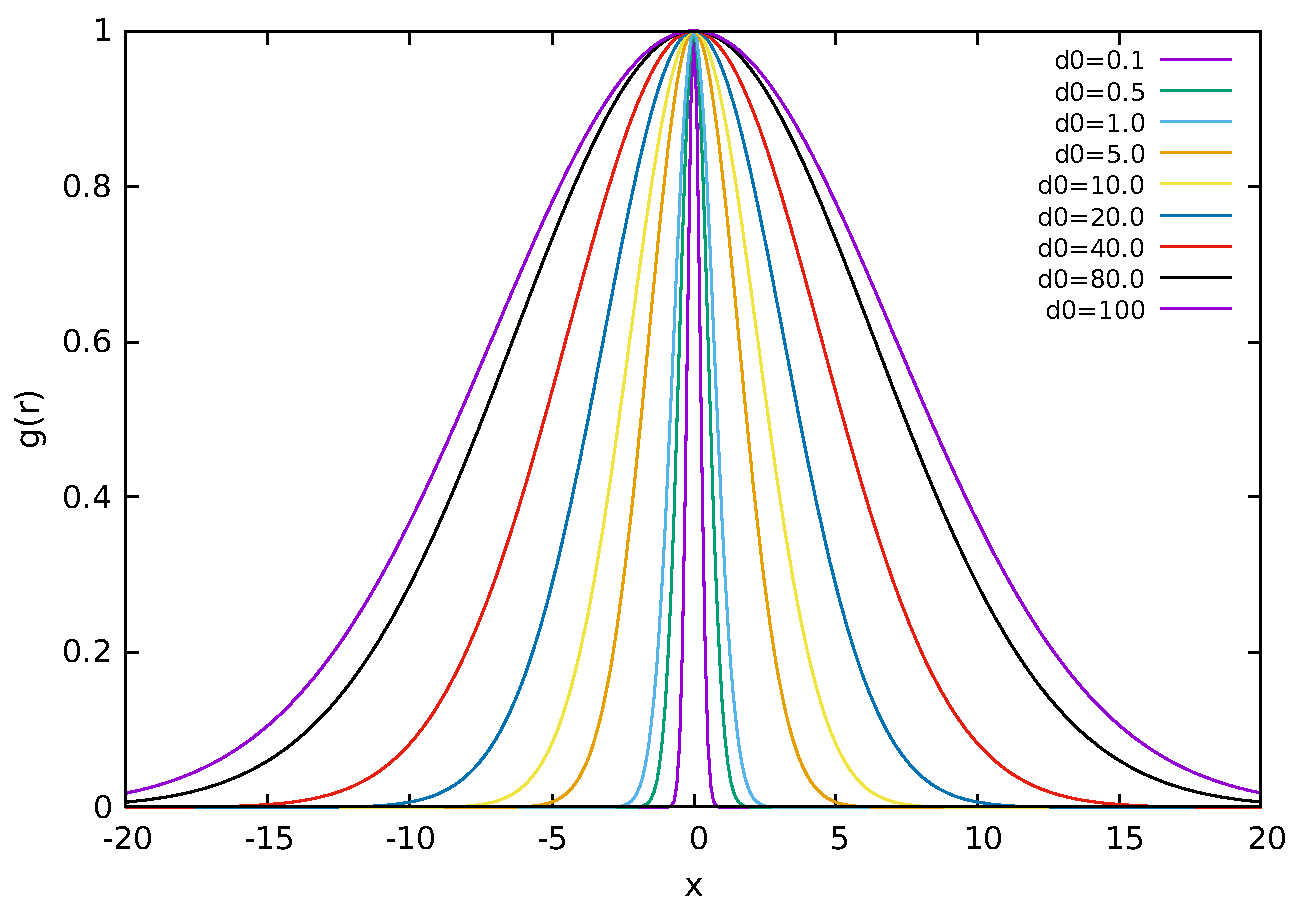
\includegraphics[width=0.7\textwidth, 
    height=0.41\textwidth, scale=1]{Gaussian_RBF.pdf}
    \caption{$g(χ)$ RBF shape for various $d_{0}$ values 
    when $χ \in [-20, 20]$}
\end{figure}

EASY built-in RBFs are described by equation \ref{RBF_equation}. In 
SMT,  
\newpage
%--------------------------------------------------------